\section{Scrambler}
\label{sec:scrambling_algorithms}

	Due to radiation levels inside the detector chamber, the main data processing takes place in a concrete bunker away from the detector.
	To facilitate this, 20 optical linkes (per modual) are used to transfer the data from the front end VELO to the Data Aquizition FPGA (DAQ).
	When comunicating data digitaly, the transfering modual (TX) and the recieving modual (RX) must have syncrinised clocks.
	In these case, the GWT serialiser is the TX, and the DAQ is the RX.
	When achieving syncronised clock, there are two main approunches:

	\begin{easylist}
		\ListProperties(Numbers=R,Margin=0.5cm,Align=fixed,FinalSpace=2em)
		% & Syncinize both the TX and RX from a single central clock - used in I$^2$C communication.
		& Transmit the TX clock with the data to the RX modual - used in I$^2$C and SPI communication.
		& Use bit-changes in the data to continuously synchronise the RX clock.
	\end{easylist}

	The former of these options, although widely used in convertional electronics, requires a finely tuned clock accounting for all possible delays.
	The latter, while negating cons of the former, requires data with a high density of tranitions to reduce the likelyhood of a desyncronisation event.
	Becuase delays in the data are possible, the latter option has been selected.

	A it is nessesary to ensure that the data has large density of transitions before being transmitted from the front-end detector to the DAQ modual.
	However, as the majority of super pixel hitmaps are empty, the data has a bais towards \textit{`0'}s.
	This reduces the frequancy of transitions in the data - increasing the probability of a desyncronisation event.
	It is therefor nesseccary to scramble the data prior to transmition and descramble the data in the DAQ FPGA.
	\par
	Scrambling and later descrambling the data is not a trivial exercise.
	The scrambleing (TX) modual and descrambling (RX) modual must use a sycronised \textit{`key'}, that is used in both the scrambling and descrambling processes.
	In the FPGA, the \textit{`key'} is derived from the previous states of the data.
	There are two methods when generating this \textit{`key'}:

	\begin{description}
		\item[Additive] The \textit{`key'} is generated by evolving the previous \textit{`key'} at each itteration of data using the incoming frame.
		\item[Multiplicative] The  \textit{`key'} is generated from the previos $n$ frames. (Here $n$ is a variable specific to the algorithm).
	\end{description}

	\subsection{Scrambler Options}
	\label{sub:scrambler_options}

		Three scrambling algorithums have been concidered:

		\begin{description}
			\item[Additive Scrambler] \hfill \\
				This scrambler is was origionally impremented and used two sets of two-input XOR logic gates.
				As the name implies, this scrambler used additive key generation which is dependent all previous input frames since the last reset signal.

			\item[Intermediate Scrambler] \hfill \\
				Created by Karol Hennessy, and deriving its name arbitrarily from the order of concideration, this multiplicative scramber combines the current and previous frames to generate the \textit{`key'}.
				Therefor, in the event of desyncronisation, only two frames are lost before the \textit{`key'} is automatically recovered.
				This feature alone is a significant improvment over the Additive Scrambler.

			\item[VeloPix Scrambler] \hfill \\
				This is the current implemented scramble algorithum in the DAQ and VeloPix code.
				Like the Intermediate Scrambler, it uses multiplicative \textit{`key'} generation.
				However, the VeloPix scrambler is compatible with further constraints enforced by the ASIC, including the number of combinational logic operations.
				The Intermediate Scrambler was design purely for simulation purposes and as such does not meet these constraints.
		\end{description}


	\subsection{Cross Checks} % (fold)
	\label{sub:cross_checks}
		The main priority when scrambling data, is ensuring that the data is recoverable.
		For all three scramblers, the algorithum was synthesised in Quartus\supercite{ref:quartus} and simulated in Modelsim\supercite{ref:modelsim}.
		The aim of synthesising and simulating the scramblers in these programs was to ensure that the design was both physical in term of on-board logic gates, and to check that the scrambled data was recoverable, respectively.
		\par
		Furthermore, a C++ simulation was created for the three scramblers.
		This simulation had two main purposes:
		firstly to cross check the output of the C++ against the Modelsim simulations;
		secondly to simulate the scrambler over a much larger simple of data as Modelsim simulations are less time effecient.
		In attition to the cross checks, the C++ code allowed for the injection of a descrnonisation event, in which the \textit{`key'} is lost.
		As expected, the Additive Scarmbler was unable to recover any data post descrnonisation, however the intermediate and VeloPix scarmblers both recovered the \textit{`key'} after two frames and continioud to recover data.

	% subsection cross_checks (end)

	\subsection{Algorithm Analysis}
	\label{sub:algorithm_analysis}

		For analytical purposes, it is assumed that fully scrambled data is indistinguisable from randomly generated data. 
		For this reason, the three algorithm are not only tested against eachother and the pre-scrambled QWT data but also randomly generated binary.
		The randomly generated data was created using the Python \textit{`random'} library, selecting a \textit{`0'} or \textit{`1'} with equal probubility.
		While the Python \textit{`random'} library is only sudo-random, on the scale of this example (i.e. $>>$ 100,000 frames), it is by far sufficient.
		\par
		A more mathematically rigorus approuch, however, is to evaluate the system abstractly in the framework of statistical physics.
		In this abstraction, the 120 bit frame (with the header and parity removed)  is concidered an ensemble; 
		microstates are the particular form of the frames;
		and macroscopic quantities can be calculated by averaging a large number of frames (i.e. the desync data).
		For the analysis outlined in section \ref{subsub:messurements_of_the_algorithms}, predictions will be made using these principles and outlined in section \ref{subsub:statistical_predictions}.
		\par
		In the context of the statisical model, it is reasonable to concider the degree of \textit{`scrambled-ness'} analogous to entropy.	This analogy is not disimular to the common interpritation of entropy as a measure of dissorder.

		\begin{equation}
			S \sim ln(\Omega)
			\label{eqn:boltzman}
		\end{equation}

		where $\Omega$ is the number of microstates assosiated with the macrostate, we learn that this state of maximum entropy is a macrostate with the maximum number of assosiated microstates.
		\par
		The entropic argument of Equation~\ref{eqn:boltzman} is not only mathematical founded. 
		For a scramble algorithum to hold for all possible data sets, it must also be capable of outputing all possible permutations. 
		As such, assuming all possible output are equally likely, the count of each macroscopic output will be proportional to the number of microstates assosiated.

		\subsubsection{Messurements of the Algorithms} 
		\label{subsub:messurements_of_the_algorithms}

			To compare the effecincy of the three algorithums in section \ref{sub:scrambler_options}, the algorithums where run over the same unput data and compared for the following measures:

			\begin{description}
				\item[Number of Transitions Per Frame] \hfill \\
					This meassure counts the total number of bit transitions (i.e. $bit(n) \neq bit(n-1)$) in a 120 bit frame. 
					The header and parity information was not included as they are not scrambled.
					This is an important test as one of the roles of the scrambler is to maximise the number of transitions.

				\item[Common Bit Chain Length] \hfill \\
					One of the downfalls of the `Number of Transitions Per Frame' analysis is that the two hypethetical 20 bit frames,

					\begin{enumerate}[a)]
						\item \textsc{10101010101111111111},
						\item \textsc{10011001100110011001},
					\end{enumerate}

					both with 10 transitions, are concidered equaly. However, (b) is clearly a more suitable output for data transfer as (a) has a large probability of desyncronisated due to the long chains of \textit{`1'}s in the right most bits.
					It is therefore also nessecary to evaluate the length of common bit chains within the scrambled data as shorter chains are more suitable for data transfer.

				\item[Bit Asymetry] \hfill \\
					Pre-scramble, the data had a large bais towards \textit{`0'}s due to the majority of the hitmaps being empty.
					Scrambled data, via entropic arguments, \textit{should} show zero bias eitherway.
					Therefor, by investigating how the number of \textit{`1'}s - \textit{`0'}s evolves over many frames, any bias in the scrambler can be found.

			\end{description}	

		\subsubsection{Statistical Predictions} % (fold)
		\label{subsub:statistical_predictions}

			\begin{description}
				\item[Number of Transitions Per Frame] \hfill \\
					
					Consider a particle in a symmetric, descrete time-dependent, two state system,

					\begin{equation}
						p_0(t) = p_1(t) = 0.5 \quad : \quad \forall\ t \in \mathbb{N},
					\end{equation}

					At each time itteration,

					\begin{equation}
						p_{i \to j}(t) = 0.5 \quad : \quad i,j = [0\ 1], \quad \forall\ t \in \mathbb{N}.
					\end{equation}

					However, assuming zero bias and detailed balance, as $p_{1 \to 0}(t)$ is equal in both probalility and importance to $p_{0 \to 1}(t)$, the probability of a bit change shall herefore be refered to as $p_{\tau}(t)$.
					\par
					Over a $n$ step process, analogous to a $n$ bit frame, the probalility distribution of the number of transitions $N_\tau$ is given by Binomial statistics,

					\begin{equation}
						f(N_{\tau}) = \frac{n!}{N_{\tau}!(n-N_{\tau})!}\ p^{N_{\tau}}\ (1 - p)^{n-N_{\tau}}
					\end{equation}

					Simplified for the special case $p = p_{\tau} = 0.5$,

					\begin{equation}
						f_{\tau}(N_{\tau}) = \frac{n!}{N_{\tau}!(n-N_{\tau})!}\ (p_{\tau})^{n}
						\label{eqn:transition_propability_dencity}
					\end{equation}

					For $n = 120$, we can calulate,

					\begin{equation}
						<N_\tau>^{Binomial} \ = \sum_{N_{\tau}=0}^{n-1} N_{\tau}\ f(N_{\tau}) = n\ p_{\tau} = 60
						\label{eqn:tansition_expectation}
					\end{equation}

					\begin{equation}
						\sigma_{N_\tau}^{Binomial} = \sqrt{ n\ p_{\tau}^2} = 5.48
					\end{equation}

					Furthermore, when concidering the entropic argument in section \ref{sub:algorithm_analysis} equation \ref{eqn:boltzman}, the number of microstates corespoding to each macrostate $N_\tau$ can be related to equation \ref{eqn:transition_propability_dencity},

					\begin{equation}
						\Omega_\tau \sim \frac{n!}{N_{\tau}!(n-N_{\tau})!}
					\end{equation}

					\begin{equation}
						<N_\tau>^{Entropic} = MAX[S_\tau] = MAX[\Omega_\tau]
					\end{equation}

					This can be numerically solved,

					\begin{equation}
						<N_\tau>^{Entropic}\ = 60
						\label{eqn:n_t_entropic}
					\end{equation}

					While the result of equation \ref{eqn:n_t_entropic} does not contibute anything new, it is important as a \textit{`sanity check'}.
					Because the system can be described as in section \ref{sub:algorithm_analysis}, it would indicated a problem in the theoretical framework if the result did not match.


				\item[Common Bit Chain Length] \hfill \\
					
					The probability of a chain of length $n$ is,

					\begin{equation}
						p_n = p_1(1 - p_\tau)^{n-1}, \quad : \quad n \in \mathbb{N}, \quad n > 1
					\end{equation}

					where $p_1$ is the number of chains of lenght 1. 
					As $p_1 = N_0 (1 -p_\tau)$, where $N_0$ is the total number of chains,

					\begin{equation}
						\frac{N_n}{N_0} = (1 - p_\tau)^n, \quad : \quad n \in \mathbb{N}, \quad n > 1
					\end{equation}

					where $N_n$ in the number of chains of length $n$.
					Takeing the log of both sides,

					\begin{align}
						log\left(\frac{N_n}{N_0}\right) &= n\ log(1 - p_\tau), \nonumber \\
 						log(N_n) &= n\  log(1 - p_\tau) + log(N_0).
 					\end{align}

					Therefor, for a graph of $log(N_n)$ against $n$ for a large sample of data, the gradient would be $log(1 - p_\tau)$.
					In this case, as $p_\tau = 0.5$, 

					\begin{equation}
						log(1 - p_\tau) = -0.30\ .
						\label{eqn:log_chain_length_gradient}			
					\end{equation}

				\item[Bit Asymetry] \hfill \\
					
					$A_{1,0}$, the assymetry of \textit{`1'}s and \textit{`0'}s is defined as,

					\begin{equation}
						A_{1,0} = N_1 - N_0,
						\label{eqn:a_def}
					\end{equation}

					where $N_1$ and $N_0$ are the number of \textit{`1'}s and \textit{`0'}s respectively.
					We can concider the evolution of $A_{1,0}$ with frame $t$ of size $n$ as a stockastic itterative map with zero deterministic growth \cite{ref:stockastic_physics},

					\begin{equation}
						A_{1,0}(nt + n\ \Delta t) = A_{1,0}(nt) + \mathcal{N}(nt)
					\end{equation}

					Where $\mathcal{N}$ is an independant random variable picked from a gausian distribution. While $A_{1,0}(t) \in \mathbb{Z}$, in the limit of large $nt$ we can approximate that $A_{1,0}$ is continious. 
					\par
					If we concider the moments of $A_{1,0}$,

					\begin{align}
						\label{eqn:A_moment1}
						<A_{1,0}(nt = M\ n\ \Delta t)> & = \sum_{m = 0}^{M -1}  \mathcal{N}(m\ n\ \Delta t), \\
						\label{eqn:A_moment2}
						<A_{1,0}(nt = M\ n\ \Delta t)^2> & = \sum_{m=0}^{M-1} \sum_{m'=0}^{M-1}  \mathcal{N}(m\ n\ \Delta t) \mathcal{N}(m'\ n\ \Delta t)\ \delta_{mm'} \nonumber \\
						&= \sum_{m=0}^{M-1} < \mathcal{N}(m\ n\ \Delta t)^2 >.
					\end{align}

					Clearly, in Equation \ref{eqn:A_moment1}, $<A_{1,0}> = 0$. In Equation \ref{eqn:A_moment2}, we assume the variance is of form $(n\ \Delta t)^\alpha$ \cite{ref:stockastic_physics}. Then,

					\begin{equation}
						<A_{1,0}(nt = M\ n\ \Delta t)^2>\ = M (n\ \Delta t)^\alpha.
						\label{eqn:A_moment3}
					\end{equation}

					Running the analysis over the frames $t = 0$ to $t_f$, the number of bits sampled is $M = {t_f / n\ \Delta t}$. Substituting this into Equation \ref{eqn:A_moment3},

					\begin{equation}
						<A_{1,0}(nt = M\ n\ \Delta t)^2>\ = t_f\ (n\ \Delta t)^{\alpha -1}.
					\end{equation}

					Concidering the three cases of $\alpha$ in the approximation of continious $n \Delta t$:
					
					\vspace{1em}

					\begin{easylist}[itemize]
						% \ListProperties{Margin=2cm,Align=fixed,FinalSpace=2em}
						& $\bm{\alpha > 1}$: Here $A_{1,0} \to 0$ as $\Delta t \to 0$.
						& $\bm{\alpha < 1}$: Here $A_{1,0} \to \infty$ as $\Delta t \to 0$.
						& $\bm{\alpha = 1}$: This is the only sensible choice.
					\end{easylist}
					
					\vspace{1em}

					With $\alpha =1$,

					\begin{equation}
						<A_{1,0}(nt = M\ n\ \Delta t)^2> = M (n\ \Delta t).
					\end{equation}

					And thus,

					\begin{equation}
						\sigma_{A_{1,0}} = \sqrt{<A_{1,0}^2> - <A_{1,0}>^2} = \sqrt{<A_{1,0}^2>} = \sqrt{n\ \Delta t}.
					\end{equation}

			\end{description}	

		\subsubsection{Results of Analysis}
		\label{subsub:algorithm_results}
			\vspace{-7mm}
			\begin{figure}[h]
				\centering
				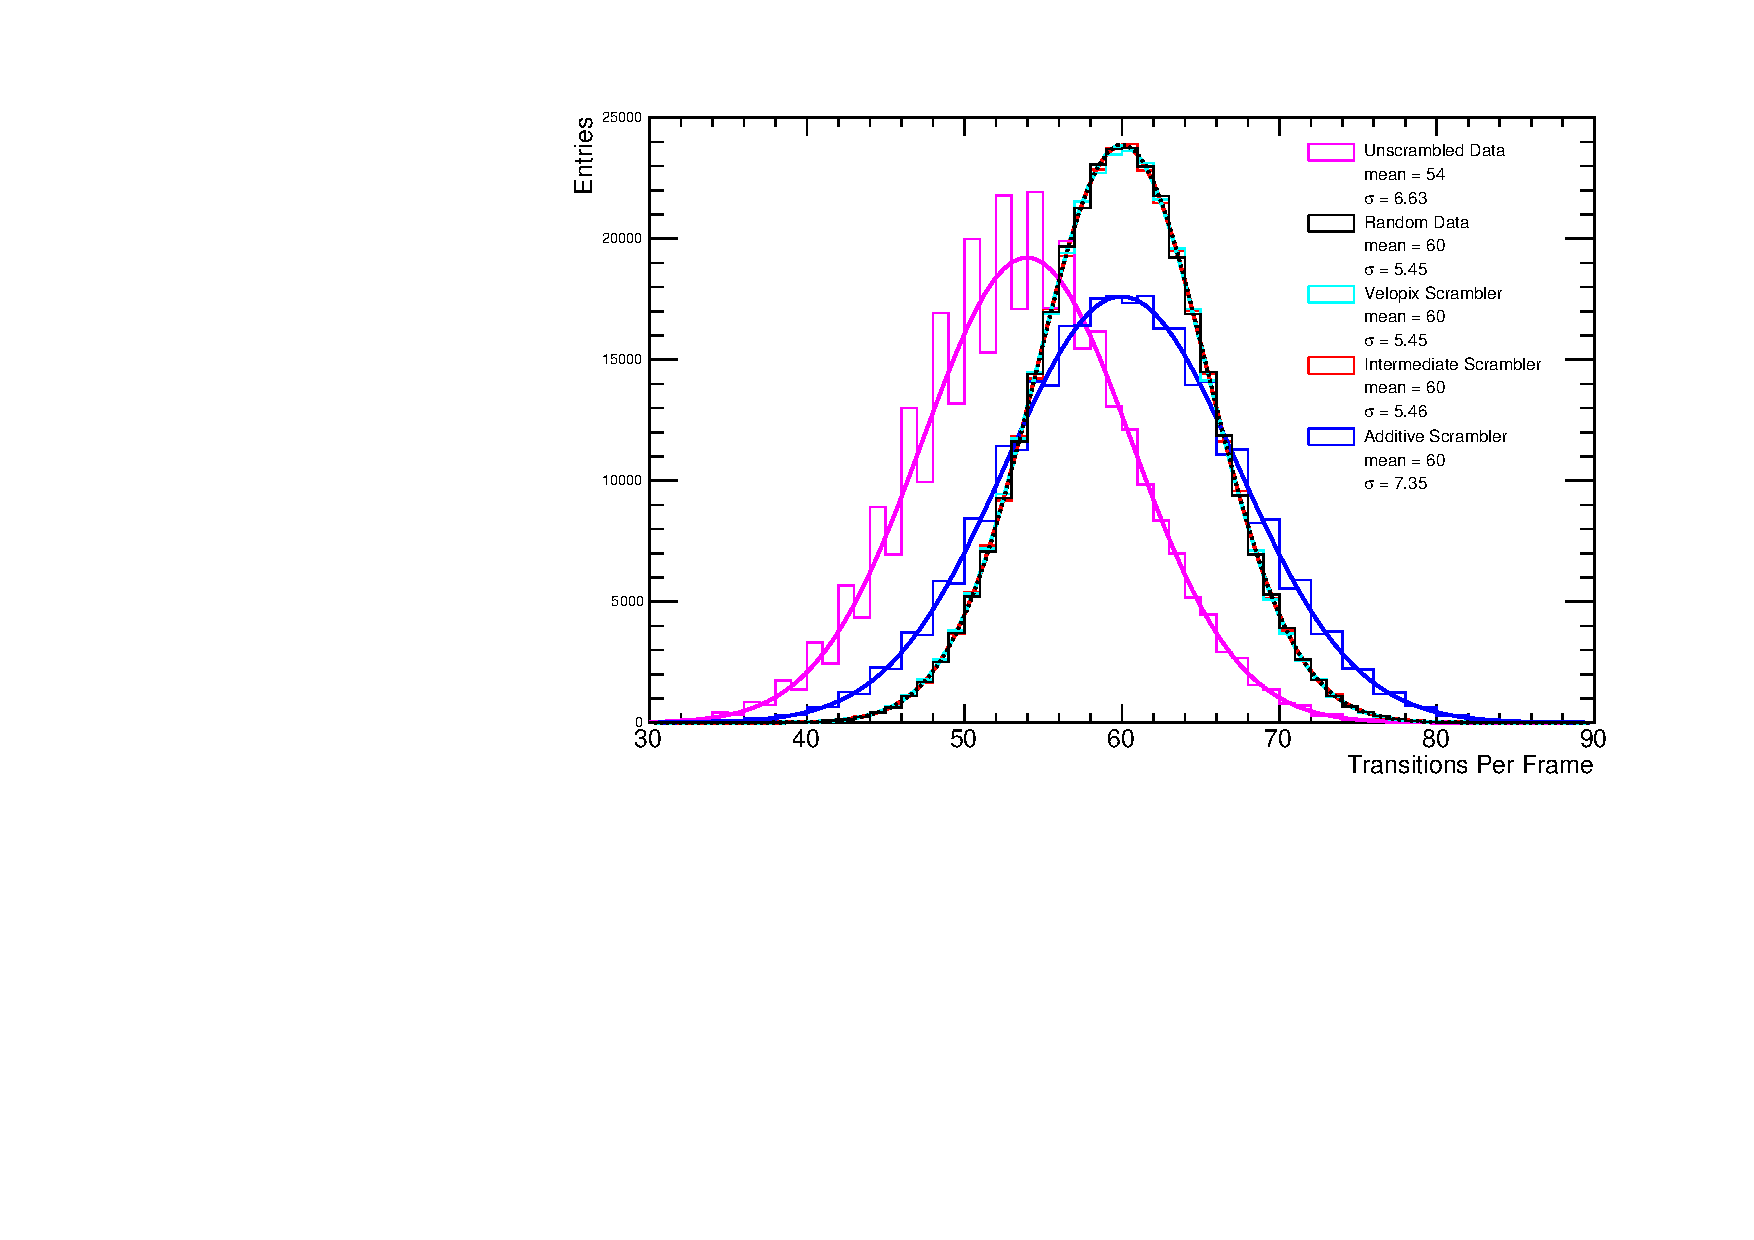
\includegraphics[width=0.75\textwidth]{Transition_Histogram_update}
				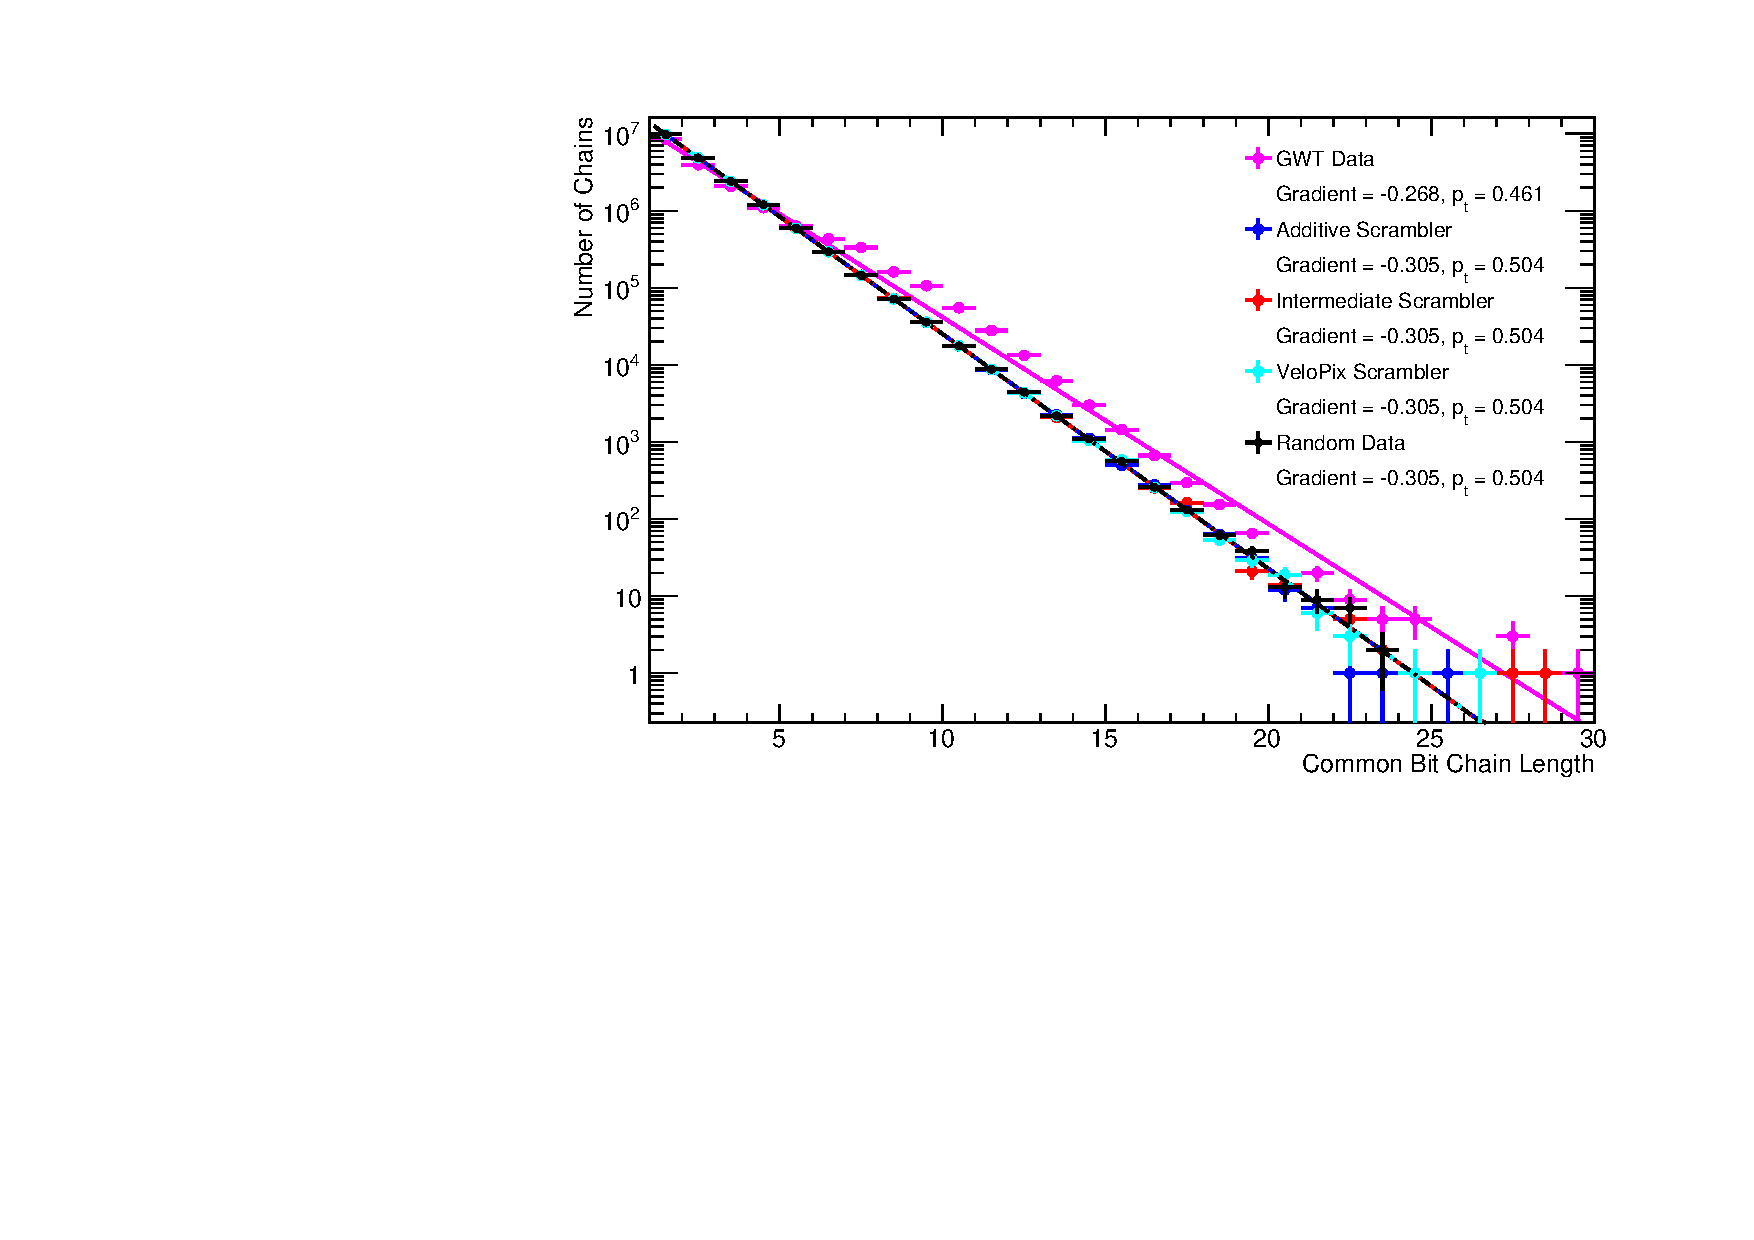
\includegraphics[width=0.75\textwidth]{Chain_length}
				\caption{Results of the \textit{`Number of Transitions Per Frame'} analysis (Top) and the \textit{`Common Bit Chain Length'} analysis (Bottom). The results for the Random Data, Intermediate Scrambler and VeloPix Scrambler overlap for the \textit{`Number of Transitions Per Frame'} analysis. The results for the Random Data, Additive Scrambler, Intermediate Scrambler and VeloPix Scrambler approximatly overlap for the \textit{`Common Bit Chain Length'} analysis.}
				\label{fig:transitions_per_frame}
			\end{figure} \FloatBarrier
			
			The results from the \textit{`Number of Transitions Per Frame'} analysis, shown in Figure~\ref{fig:transitions_per_frame}, show a strong corelation between the Intermediate and VeloPix Scramblers with the randomly generated data. 
			These results are withing 1\% agreement with the theoretical predictions for $<N_\tau> = 60$ and $\sigma_{N_\tau} = 5.48$, made in Section~\ref{subsub:statistical_predictions}. 
			The remarkable consistancy between the theoretical predictions and the randomly gernerated data provides confidance in both the theory, and the scrambled nature of the Intermediate and VeloPix scrambler outputs.
			\par		
			 All three scramblers, the random data, and the theoretical predictions are all consistant to within 1\%. 
			 Comparing the two results for the Additive Scrambler, its shown that while the frequancy of longer chains is consistant with random data; but as the variance of transitions is larger than predicted, the long and short trains are more localy clustered. 

			\begin{figure}
				\centering
				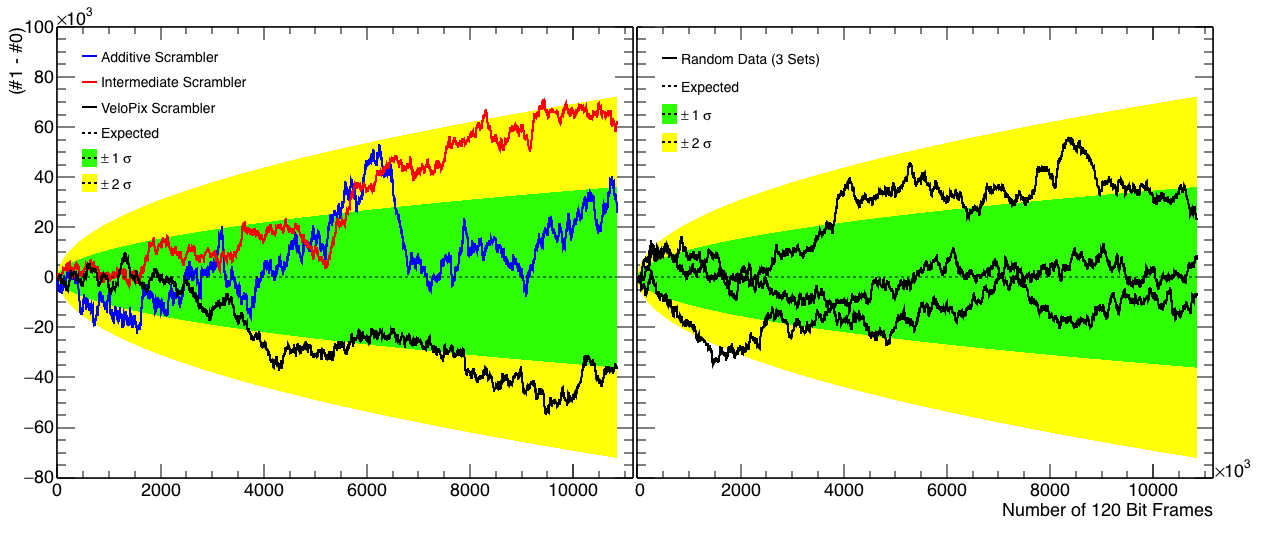
\includegraphics[width=1\textwidth]{Balance_graph_cropped}
				\caption{The results of the \textit{`Bit Asymetry'} analysis.}
				\label{fig:bit_asym}
			\end{figure}

			The \textit{`Bit Asymetry'} of each scrambler, shown in Figure~\ref{fig:bit_asym}, is consistant with the theoretical prediction. 
			The deviation of $A_{1,0}$ for the predicted mean of 0 is fully consistant with stockastic noise. 
			The random data also shows consistancy. 
			This gives confidance in the assumtpions made in Section~\ref{subsub:statistical_predictions}.		
 			\par		
 			One notible feature of Figure\ref{fig:bit_asym} is the steap grandient of the additive scrambler a $t \sim 6.10^6$.		
 			However, as the data stays within the theoretical limits and the \textit{`drop'} is of approximatly $\Delta A_{1,0} \sim 60.10^3$ over the range $n\ \Delta t \sim 1.2.10^8$ it would be difficult to construnct any argument claiming that this feature is of statistically significance		
 			\par		
 			\textbf{(I am tempted to run $\chi^2$ analysis for a fit of y=0 so show that the data the data is consistant with the model, but am nut sure this will actually add to the argument?)}

	\subsection{Conclusion}

		\begin{table}[h]		
 			\centering		
 			\begin{TAB}(r)[7pt]{l|cc:cc}{c|c:ccc:cc}		
 							           & $<N_\tau>$ & $\sigma_{N_\tau}$ & Gradient  	& $p_\tau$    \\		
 				GQT data  		       & 54      	& 6.63           	& -0.268 		& 0.460 \\		
 				Additive Scrambler     & 60      	& 7.35           	& -0.305 		& 0.504 \\		
 				Intermediate Scrambler & 60      	& 5.45           	& -0.305 		& 0.504 \\		
 				Velopix Scrambler      & 60      	& 5.46           	& -0.305 		& 0.504 \\		
 				Random Data            & 60      	& 5.45           	& -0.305 		& 0.504 \\		
 				Theoretical Prediction & 60      	& 5.48           	& -0.3 			& 0.5   			
 			\end{TAB}		
 			\caption{The combined results of the algorithum analysis.}		
 			\label{tab:comb_results}		
 		\end{table}		
 		
 		The consistancy of random data and the theoretical predictions justifies the assumptions and approximations made in Section~\ref{sub:algorithm_analysis} and Section~\ref{subsub:statistical_predictions}. 
 		Furthermore, the conformation of the statistical model allows for accurate comparisons to be made form predicted values and their measured counterparts.		
 		\par		
 		The Additive Scrambler, while consistant with the \textit{`Chain Length'} and \textit{`Bit Asymetry'} analysis, has a variance in the transition frequancy that leads the concultion that long and short chains are locally clusted. 		
 		This is not ideal for data transfer. 		
 		Many sequenchal long chains increase the probability of TX-RX clock desycronisation. 		
 		Furthermore, the additive scrambler will not recover from this loss of syncronisation, as the \textit{`key'} will never be recovered without a common reset signal.		
 		\par		
 		The Intermediate Scrambler produced an output consistant with random data. 		
 		This makes the algorithm suitable of data transfer.		
 		As already mentioned\footnote{Note to Marco: this is in the scrabler options section}, however, the scrambler is designed for computer simulated.		
 		As such, it is not suitable for implementation as it does not meet the additions requirments of the ASIC.		
 		\par		
 		The VeloPix Scrambler, like the Intermediate Scrambler, produces a statistically scrambled output.		
 		Furthermore, the algorithum in inline with the additional requirments of the ASIC.		
 		As such, it ideal for implementation, and hense is currently the choice algorithum for use in the 2019 VELO upgrade.